\documentclass[11pt,a4paper]{ctexart}
\usepackage{geometry}
\usepackage{graphicx}
\usepackage{subfigure}
\usepackage{amsmath}
\usepackage{multirow}
\usepackage{listings}
\usepackage{verbatim}
\usepackage[colorlinks, linkcolor=black, anchorcolor=black, citecolor=black]{hyperref}

\CTEXsetup[format={\Large\bfseries}]{section}
\geometry{left=1in, right=1in, top=1in, bottom=1in}
\begin{document}
\title{数值分析与算法 \hspace{0.1in} 大作业1}
\author{罗云鹏 \hspace{0.1in} 自 64 \hspace{0.1in}2016011470}
\maketitle
\tableofcontents
\newpage

\section{采用数值方法求$\pi$}
由微积分知识可知
$$\int_0^1\dfrac{1}{1+x^2}dx = arctan(x)\bigg|_0^1 = \dfrac{1}{\pi}$$
使用数值积分方法求$4 \times \int_0^1\dfrac{1}{1+x^2}$即可求得$\pi$的值。

使用复化梯形公式求积分,计算公式如下
$$\pi = 4 \times \dfrac{h}{2}\left[f(0) + 2\sum\limits_{k=1}^{n-1}f(kh) + f(1)\right]$$
其中$h = \dfrac{1}{n}$。

\subsection{计算代价和收敛速度}
在计算过程中,浮点数乘法相对于加法的计算代价大得多,故只分析乘法的次数。
在计算$2 \times \dfrac{1}{x^2+1}$时,共有4次乘法,而一共约有$n$次计算,故乘法次数约为$4n$。
若取$n=10^6$,那么乘法次数约为$4\times 10^6$次。

算法空间代价为$O(1)$。

\subsection{误差分析}
\subsubsection{截断误差}
算法的截断误差限为$R[f] = - \dfrac{(b-a)^2}{12}h^2f''(\xi)$,又有积分范围为$[0, 1]$,$f''(x) \le 2$,则有
$$R[f] \le \dfrac{1}{6}h^2$$

\subsubsection{存储误差}
使用双精度浮点数,有效数字为$15$位。
计算$\dfrac{1}{1+x^2}$时,存储误差来源为:
\begin{itemize}
    \item $x$本身存储误差$0.5 \times 10^{-15}$。
    \item 计算$x^2$时,上一步累积误差及结果存储误差,共$1.5 \times 10^{-15}$。
    \item 计算$1 + x^2$时,上一步累积误差及结果存储误差,共$1.5 \times 10^{-15} + 0.5 \times 10^{-14} = 0.65 \times 10^{-14}$。
    \item 计算$\dfrac{1}{1 + x^2}$时,上一步累积误差及结果存储误差,共$0.65 \times 10^{-14} \times \max\limits_{x\in[0, 1]}\left(\dfrac{1}{1+x^2}\right)' + 0.5 \times 10^{-15} \le 1 \times 10^{-14}$。
\end{itemize}

求和后,易分析得存储误差小于$1\times10^{-13}$。

若取$n = 10^6$,则总误差满足$\Delta \le 2.4 \times 10^{-13}$。

\section{采用数值方法求$\ln(\pi)$}
对$\ln(x)$在$x = 1$处进行泰勒展开,可得
$$\ln(x) = \sum\limits_{i = 1}^{\infty} (-1)^{i-1} \dfrac{(x-1)^i}{i}$$
若取前$n$项进行计算,收敛域为$x \in (1, 2)$,则有公式
$$\ln(x) \approx \sum\limits_{i = 1}^{n} (-1)^{i-1} \dfrac{(x-1)^i}{i}$$

根据对数特性,把计算$\ln(\pi)$化为计算$\ln(\dfrac{\pi}{1.25^4}) + 4\ln(1.25)$。
使用上述公式分别计算$\ln(\dfrac{\pi}{1.25^4})$ 和 $\ln(1.25)$,即可求得$\ln(\pi)$。

\subsection{计算代价和收敛速度}
对于$\sum\limits_{i = 1}^{n} (-1)^{i-1} \dfrac{(x-1)^i}{i}$中的第$i$项,需要计算$i+2$次乘法,对于整个计算过程来说,则总共有$\dfrac{n(n+5)}{2}$次乘法。
若取$n=24$,那么乘法次数为$348$次。

算法空间代价为$O(1)$。

\subsection{误差分析}
\subsubsection{截断误差}
截断误差为
$$R = \sum\limits_{i = n+1}^{\infty} (-1)^{i-1} \dfrac{(x-1)^i}{i} \le \dfrac{(x-1)^{n+1}}{n+1}$$

取$n=24$,又有$\dfrac{\pi}{1.25^4}, 1.25 < 1.3$,则可得
$$R < \dfrac{0.3^{25}}{25} < 3.4\times 10^{-15}$$

\subsubsection{存储误差}
使用双精度浮点数,有效数字为$15$位。
计算$\dfrac{1}{i}(x-1)^i(-1)^{i-1}$时,存储误差来源为:
\begin{itemize}
    \item $x-1$存储误差为$0.5\times 10^{-15}$。
    \item 计算$\dfrac{1}{i}(x-1)^i(-1)^{i-1}$时,上一步存储误差累计为$\left(\dfrac{1}{i}(x-1)^i(-1)^{i-1}\right)' \times 0.5\times 10^{-15} \le 0.5\times 10^{-15}$
\end{itemize}

求和后,存储误差为$n\times 0.5 \times 10^{-15} = 1.2 \times 10^{-14}$。

\subsubsection{之前计算结果误差累计}
计算$\ln(\dfrac{\pi}{1.25^4})$时,会受到来自上一步的误差影响。
$\Delta_{\pi}' = \Delta(\dfrac{\pi}{1.25^4}) < \Delta_{\pi} + 0.5\times 10^{-14} < 2\Delta_\pi$。那么累积误差为

$$\left(\sum\limits_{i = 1}^{n} (-1)^{i-1} \dfrac{(x-1)^i}{i}\right)' \times \Delta_\pi' \le \dfrac{(x-1)^1}{1} \times \Delta_\pi' \le \Delta_\pi$$

综上,总误差为
$$\Delta_{\ln(\pi)} = 5 \times 3.4\times 10^{-15} + 5 \times 1.2\times 10^{-14} + 2.4 \times 10^{-13} \le 3.2\times 10^{-13}$$

\section{采用数值方法求$\pi^x$}
由第二步,已经求得$\ln(\pi)$,则计算$e^{x\ln(\pi)}$即可得到$\pi^x$的值。

有$(e^x)' = e^x$,则可使用求解常微分方程的方法计算结果。
采用改进的欧拉法,
\begin{align*}
    &\bar{y}_{n+1} = y_n + hf(x_n, y_n) \\
    &y_{n+1} = y_n + \dfrac{h}{2}\left[f(x_n, y_n) + f(x_{n+1}, \bar{y}_{n+1})\right]
\end{align*}
其中$h = \dfrac{x}{n}, y_0 = 1$。
有$f(x_n, y_n) = e^{x_n} = y_n$,整理上式后有
$$y_{n+1} = (1 + h + \dfrac{h^2}{2})y_n$$

\subsection{计算代价和收敛速度}
计算前,将$(1+h+\dfrac{h^2}{2})$预先计算并存储,迭代时作为一个常量。
每次迭代时需要计算一次乘法。
若取$n = 10^7$,那么共需要计算$10^7$次乘法。

算法空间代价为$O(1)$。


\subsection{误差分析}
\subsubsection{方法累积误差}
改进欧拉法的方法误差满足
$$\Delta_{n+1} \le (1 + hM + \dfrac{h^2}{2}M^2)\Delta_n + (\dfrac{LM}{4}+\dfrac{T}{12})$$
其中$\lvert\dfrac{\partial f}{\partial y}(x, y)\rvert \le M$,$\lvert y^{(2)}(x)\rvert \le L$,$\lvert y^{(3)}(x)\rvert \le T$。
根据$f(x, y) = e^x$,可取$M = 1, L = T = 10^5 < \max\limits_{x\in(1, 10)}e^x$。

可将方法误差求出
$$\Delta_n \le \left((1+h+\dfrac{h^2}{2})^n-1\right)(\dfrac{2Lh^2}{6+3h}) \le \dfrac{2}{3}Lh^2 = \dfrac{2}{3} \times 10^5 h^2$$

\subsubsection{存储误差}
在程序中使用\_\_float128类型的浮点数,其十进制有效位数为34位。

由于$y_n < 10^5$,在计算$y_{n+1} = (1+h+\dfrac{h^2}{2})y_n$时,每步可能会产生$0.5 \times 10^{-28}$大小的存储误差。
使用与方法误差相同的分析方法,可求出$\delta_n < (1+h+\dfrac{h^2}{2})^n(\dfrac{0.5\times 10^{-28}}{h+\dfrac{1}{2}h^2}) < \dfrac{3\times 0.5 \times 10^{-28}}{h}$。

\subsubsection{累积误差}
显然有
$$x\Delta_{\ln(\pi)} \le 10 \Delta_{\ln(\pi)} \le 3.2 \times 10^{-12}$$
那么使用相似的方法,可以计算得到
$$\Delta \le (1+h+\dfrac{h^2}{2})^n \times x\Delta_{\ln(\pi)} \le 3 \times 10 \times 3.2 \times 10^{-12} \le 10^{-10}$$


总误差为
$$\Delta \le \dfrac{2}{3}\times 10^5 h^2 + \dfrac{0.15\times 10^{-28}}{h} + 10^{-10}$$
取$n = 10^7$,那么$h = \dfrac{x}{n} \in [10^{-7}, 10^{-6}]$,则有
$$\Delta \le 0.7 \times 10^{-7} < 0.5 \times 10^{-6}$$
满足要求。

\clearpage

\section{程序框图}
程序三步分别编写为函数,其程序框图如\ref{fig:pic}

\begin{figure}[H]
    \begin{center}
        \subfigure[计算$\pi$]{
            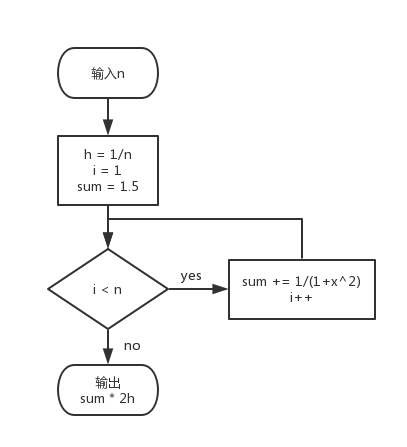
\includegraphics[width=0.46\textwidth]{pic/pi.png} }
        \subfigure[计算$\ln$]{
            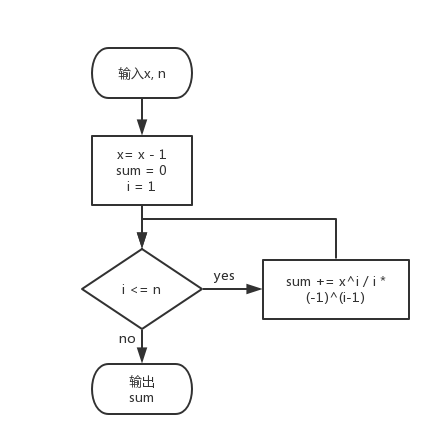
\includegraphics[width=0.46\textwidth]{pic/ln.png} }
        \subfigure[计算$e^x$]{
            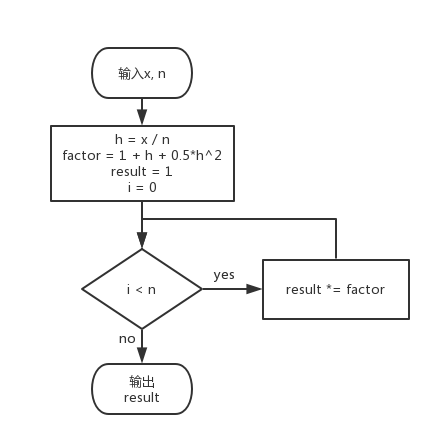
\includegraphics[width=0.46\textwidth]{pic/exp.png} }
    \end{center}
    \caption{程序框图}
    \label{fig:pic}
\end{figure}

\section{实验结果及分析}

实验结果如图\ref{fig:result}。

\begin{figure}[H]
    \begin{center}
        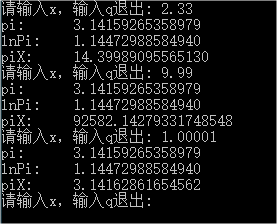
\includegraphics[width=4in]{pic/result.png}
    \end{center}
    \caption{实验结果}
    \label{fig:result}
\end{figure}

计算结果和用其他方式计算所得参考值对比如表\ref{tab:contract}。
可以看到,计算值保证了小数点后六位有效数字,当$x$偏大时,计算结果小数点后第七位可能存在一定误差。

\begin{table}[H]
    \centering
    \begin{tabular}{|c|c|c|c|}
        \hline
        x & 2.33 & 9.99 & 1.00001 \\ \hline
        计算值 & 14.3998910 & 92582.1427933 & 3.1416286 \\ \hline
        参考值 & 14.3998910 & 92582.1427935 & 3.1416286 \\ \hline
    \end{tabular}
    \caption{计算值和参考值的对比}
    \label{tab:contract}
\end{table}

通过随机生成$[1, 10)$范围内的值,对程序进行验证,其结果如下。

其中每一组数据第一排为$x$的值,第二排为计算值,第三排为参考值。
第二、三排中,第一个数字为保留14位有效数字结果,第二个为保留6为有效数字结果。
可以看出程序能保证小数点后六位有效数字。

\verbatiminput{../result.txt}

\end{document}
